%%%%%%%%%%%%%%%%%%%%%%%% editor.tex %%%%%%%%%%%%%%%%%%%%%%%%%%%%%
%
% sample root file for the contributions of a "contributed volume"
%
% Use this file as a template for your own input.
%
%%%%%%%%%%%%%%%%%%%%%%%%%%%%% Springer %%%%%%%%%%%%%%%%%%%%%%%%%%


% RECOMMENDED %%%%%%%%%%%%%%%%%%%%%%%%%%%%%%%%%%%%%%%%%%%%%%%%%%%
\documentclass[graybox, envcountchap]{svmult}

% choose options for [] as required from the list
% in the Reference Guide

\usepackage{mathptmx}        % selects Times Roman as basic font
\usepackage{helvet}          % selects Helvetica as sans-serif font
\usepackage{courier}         % selects Courier as typewriter font
%\usepackage{type1cm}        % activate if the above 3 fonts are 
                             % not available on your system

\usepackage{makeidx}         % allows index generation
\usepackage{graphicx}        % standard LaTeX graphics tool
                             % when including figure files
\graphicspath{{./},{Figures/}}
\usepackage{multicol}        % used for the two-column index
\usepackage[bottom]{footmisc}% places footnotes at page bottom

\usepackage{epstopdf}


% see the list of further useful packages in the Reference Guide

\makeindex             % used for the subject index
                       % please use the style svind.ist with
                       % your makeindex program

%%%%%%%%%%%%%%%%%%%%%%%%%%%%%%%%%%%%%%%%%%%%%%%%%%%%%%%%%%%%%%%%%

%% Added by Overleaf to facilitate author contributions in folders
\usepackage{import}



\newif\ifslo
\slotrue
%\slofalse

\ifslo
\usepackage[utf8]{inputenc}
\usepackage[slovene]{babel}
\newcommand{\fig}{Slika~}
\newcommand{\figs}{Slike~}
\newcommand{\eq}{Enačba~}
\newcommand{\eqs}{Enačbe~}
\newcommand{\tab}{Tabela~}
\newcommand{\tabs}{Tabele~}
\newcommand{\sect}{Poglavje~}
\newcommand{\sects}{Poglavja~}
\newcommand{\eng}[1]{(angl.~\emph{#1})}

\else

\newcommand{\fig}{Fig.~}
\newcommand{\figs}{Figs.~}
\newcommand{\eq}{Equation~}
\newcommand{\eqs}{Equations~}
\newcommand{\tab}{Table~}
\newcommand{\tabs}{Tables~}
\newcommand{\sect}{Section~}
\newcommand{\sects}{Sections~}

\fi




\begin{document}

\begin{otherlanguage}{slovene}
\extrachap{Analiza in načrtovanje bioloških vezij z ogrodjem GReNMlin ter ostale teme s področja biološkega procesiranja}
\large Uredila prof. dr. Miha Moškon in prof. dr. Miha Mraz\\
\\
\normalsize \emph{Januar, 2025}



%\frontmatter%%%%%%%%%%%%%%%%%%%%%%%%%%%%%%%%%%%%%%%%%%%%%%%%%%%%%%

%%%%%%%%%%%%%%%%%%%%%%%% dedic.tex %%%%%%%%%%%%%%%%%%%%%%%%%%
%
% sample dedication
%
% Use this file as a template for your own input.
%
%%%%%%%%%%%%%%%%%%%%%%%% Springer %%%%%%%%%%%%%%%%%%%%%%%%%%

\begin{dedication}
Use the template \emph{dedic.tex} together with the Springer document class SVMono for monograph-type books or SVMult for contributed volumes to style a quotation or a dedication\index{dedication} at the very beginning of your book in the Springer layout
\end{dedication}




%\include{EditorContents/foreword}
\preface

Navodila za urejanje: 
\begin{itemize}
\item Vaše datoteke se nahajajo v direktorijih \texttt{Skupina*}, kjer \texttt{*} predstavlja številko vaše skupine - glavna datoteka je texttt{main.text}.
\item Če mape za vašo skupino še, jo ustvarite.
\item Slike shranjujte v svoj direktorij.
\item Vse labele začnite z znaki \texttt{g*:}, kjer \texttt{*} predstavlja številko vaše skupine.
\item Pri referenciranju virov uporabite datoteko \texttt{references.bib}, ki se nahaja v korenskem direktoriju projekta.
\item Pred dodajanjem novih virov v datoteko \texttt{references.bib} dobro preverite, če je vir mogoče že vsebovan v datoteki - v tem primeru se sklicujte na obstoječ vnos.
\end{itemize}

Seminarska dela so osredotočena na načrtovanje in optimizacijo bioloških logičnih gradnikov implementiranimi z gensko regulatornimi omrežji. Pri tem boste izhajali iz knjižnice GReNMlin\footnote{\url{https://github.com/mmoskon/GRenMlin/}}, ki je namenjena delu s tovrstnimi gradniki. V svojih delih se lahko osredotočite na načrtovanje, analizo in optimizacijo novih bioloških logičnih vezij ali pa na razširitve predlagane knjižnice. Izberete si lahko tudi katerakoli druga orodja ali teme s področja biološkega procesiranja.

\vspace{\baselineskip}
\begin{flushright}\noindent
Ljubljana,\hfill {\it prof. dr. Miha Moškon}\\
januar, 2025\hfill {\it prof. dr. Miha Mraz}\\
\end{flushright}



%%%%%%%%%%%%%%%%%%%%%%acknow.tex%%%%%%%%%%%%%%%%%%%%%%%%%%%%%%%%%%%%%%%%%
% sample acknowledgement chapter
%
% Use this file as a template for your own input.
%
%%%%%%%%%%%%%%%%%%%%%%%% Springer %%%%%%%%%%%%%%%%%%%%%%%%%%

\extrachap{Zahvala}
TODO

%Avtorji posameznih poglavij so slušatelji predmeta \textit{Nekonvencionalne platforme in metode procesiranja}, ki se je v študijskem letu 2023/2024 predaval na 2. stopnji univerzitetnega študija Računalništva in informatike na Fakulteti za računalništvo in informatiko Univerze v Ljubljani. Vsem študentom se zahvaljujeva za izkazani trud, ki so ga vložili v svoje prispevke.

\begin{flushright}
\textit{prof. dr. Miha Moškon in prof. dr. Miha Mraz, Ljubljana, januar 2025}
\end{flushright}



\tableofcontents
%%%%%%%%%%%%%%%%%%%%%clist.tex %%%%%%%%%%%%%%%%%%%%%%%%
%                                                    
% sample list of contributors and their addresses    
%                                                    
% Use this file as a template for your own input.    
%                                                    
%%%%%%%%%%%%%%%%%%%%%%%% Springer %%%%%%%%%%%%%%%%%%%%
\contributors

\begin{thecontriblist}
Firstname Surname
\at ABC Institute, 123 Prime Street, Daisy Town, NA 01234, USA, \email{smith@smith.edu}
\and
Firstname Surname
\at XYZ Institute, Technical University, Albert-Schweitzer-Str. 34, 1000 Berlin, Germany, \email{meier@tu.edu}
\end{thecontriblist}
%%%%%%%%%%%%%%%%%%%%%%%acronym.tex%%%%%%%%%%%%%%%%%%%%%%%%%%%%%%%%%%%%%%%%%
% sample list of acronyms
%
% Use this file as a template for your own input.
%
%%%%%%%%%%%%%%%%%%%%%%%% Springer %%%%%%%%%%%%%%%%%%%%%%%%%%

\extrachap{Okrajšave}

Use the template \emph{acronym.tex} together with the Springer document class SVMono (monograph-type books) or SVMult (edited books) to style your list(s) of abbreviations or symbols in the Springer layout.

Lists of abbreviations\index{acronyms, list of}, symbols\index{symbols, list of} and the like are easily formatted with the help of the Springer-enhanced \verb|description| environment.

\begin{description}[CABR]
\item[ABC]{Spelled-out abbreviation and definition}
\item[BABI]{Spelled-out abbreviation and definition}
\item[CABR]{Spelled-out abbreviation and definition}
\end{description}


%\mainmatter%%%%%%%%%%%%%%%%%%%%%%%%%%%%%%%%%%%%%%%%%%%%%%%%%%%%%%%
%%%%%%%%%%%%%%%%%%%%%%part.tex%%%%%%%%%%%%%%%%%%%%%%%%%%%%%%%%%%
% 
% sample part title
%
% Use this file as a template for your own input.
%
%%%%%%%%%%%%%%%%%%%%%%%% Springer %%%%%%%%%%%%%%%%%%%%%%%%%%

\begin{partbacktext}
\part{Part Title}
\noindent Use the template \emph{part.tex} together with the Springer document class SVMono (monograph-type books) or SVMult (edited books) to style your part title page and, if desired, a short introductory text (maximum one page) on its verso page in the Springer layout.

\end{partbacktext}
\import{Skupina1/}{main}
\import{Skupina2/}{main}
\import{Skupina3/}{main}
\end{otherlanguage}
\import{Skupina4/}{main}
%

%\backmatter%%%%%%%%%%%%%%%%%%%%%%%%%%%%%%%%%%%%%%%%%%%%%%%%%%%%%%%
%\appendix
%%%%%%%%%%%%%%%%%%%%%% appendix.tex %%%%%%%%%%%%%%%%%%%%%%%%%%%%%%%%%
%
% sample appendix
%
% Use this file as a template for your own input.
%
%%%%%%%%%%%%%%%%%%%%%%%% Springer-Verlag %%%%%%%%%%%%%%%%%%%%%%%%%%

\chapter{Chapter Heading}
\label{introA} % Always give a unique label
% use \chaptermark{}
% to alter or adjust the chapter heading in the running head

Use the template \emph{appendix.tex} together with the Springer document class SVMono (monograph-type books) or SVMult (edited books) to style appendix of your book in the Springer layout.


\section{Section Heading}
\label{sec:A1}
% Always give a unique label
% and use \ref{<label>} for cross-references
% and \cite{<label>} for bibliographic references
% use \sectionmark{}
% to alter or adjust the section heading in the running head
Instead of simply listing headings of different levels we recommend to let every heading be followed by at least a short passage of text. Further on please use the \LaTeX\ automatism for all your cross-references and citations.


\subsection{Subsection Heading}
\label{sec:A2}
Instead of simply listing headings of different levels we recommend to let every heading be followed by at least a short passage of text. Further on please use the \LaTeX\ automatism for all your cross-references and citations as has already been described in Sect.~\ref{sec:A1}.

For multiline equations we recommend to use the \verb|eqnarray| environment.
\begin{eqnarray}
\vec{a}\times\vec{b}=\vec{c} \nonumber\\
\vec{a}\times\vec{b}=\vec{c}
\label{eq:A01}
\end{eqnarray}

\subsubsection{Subsubsection Heading}
Instead of simply listing headings of different levels we recommend to let every heading be followed by at least a short passage of text. Further on please use the \LaTeX\ automatism for all your cross-references and citations as has already been described in Sect.~\ref{sec:A2}.

Please note that the first line of text that follows a heading is not indented, whereas the first lines of all subsequent paragraphs are.

% For figures use
%
\begin{figure}[t]
\sidecaption[t]
% Use the relevant command for your figure-insertion program
% to insert the figure file.
% For example, with the graphicx style use
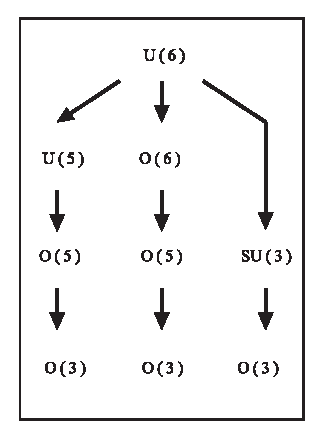
\includegraphics[scale=.65]{figure}
%
% If no graphics program available, insert a blank space i.e. use
%\picplace{5cm}{2cm} % Give the correct figure height and width in cm
%
\caption{Please write your figure caption here}
\label{fig:A1}       % Give a unique label
\end{figure}

% For tables use
%
\begin{table}
\caption{Please write your table caption here}
\label{tab:A1}       % Give a unique label
%
% Follow this input for your own table layout
%
\begin{tabular}{p{2cm}p{2.4cm}p{2cm}p{4.9cm}}
\hline\noalign{\smallskip}
Classes & Subclass & Length & Action Mechanism  \\
\noalign{\smallskip}\hline\noalign{\smallskip}
Translation & mRNA$^a$  & 22 (19--25) & Translation repression, mRNA cleavage\\
Translation & mRNA cleavage & 21 & mRNA cleavage\\
Translation & mRNA  & 21--22 & mRNA cleavage\\
Translation & mRNA  & 24--26 & Histone and DNA Modification\\
\noalign{\smallskip}\hline\noalign{\smallskip}
\end{tabular}
$^a$ Table foot note (with superscript)
\end{table}
%

%%%%%%%%%%%%%%%%%%%%%%%acronym.tex%%%%%%%%%%%%%%%%%%%%%%%%%%%%%%%%%%%%%%%%%
% sample list of acronyms
%
% Use this file as a template for your own input.
%
%%%%%%%%%%%%%%%%%%%%%%%% Springer %%%%%%%%%%%%%%%%%%%%%%%%%%

\Extrachap{Glossary}


Use the template \emph{glossary.tex} together with the Springer document class SVMono (monograph-type books) or SVMult (edited books) to style your glossary\index{glossary} in the Springer layout.


\runinhead{glossary term} Write here the description of the glossary term. Write here the description of the glossary term. Write here the description of the glossary term.

\runinhead{glossary term} Write here the description of the glossary term. Write here the description of the glossary term. Write here the description of the glossary term.

\runinhead{glossary term} Write here the description of the glossary term. Write here the description of the glossary term. Write here the description of the glossary term.

\runinhead{glossary term} Write here the description of the glossary term. Write here the description of the glossary term. Write here the description of the glossary term.

\runinhead{glossary term} Write here the description of the glossary term. Write here the description of the glossary term. Write here the description of the glossary term.


%%%%%%%%%%%%%%%%%%%%%%%%%%%%%%%%%%%%%%%%%%%%%%%%%%%%%%%%%%%%%%%%%%%%%%

\backmatter
\bibliographystyle{ieeetr}
\bibliography{references}



%\printindex

\end{document}

